\section{船闸}\label{sec:5-9}

为了充分利用河水来灌溉农田或推动水力发电机工作,往往需要在河流上修建拦河坝,提高水位。
但是,修建了拦河坝以后,河水被大坝隔断,上游水位又高于下游水位,船只就不能通过了。
在水上运输频繁的江河上,为了解决这个问题,人们利用了连通器的原理,在拦河坝的旁边修建了船闸。

船闸是从河中隔离出来的供船只通过的通道。在船闸跟上下游连接的地方各有一座闸门〈图 \ref{fig:5-34} 中的 $C$ 和 $D$),
闸门底下有输水阀门 $A$ 和 $B$,船只可以通过闸门进出船闸。

\begin{figure}[htbp]
    \centering
    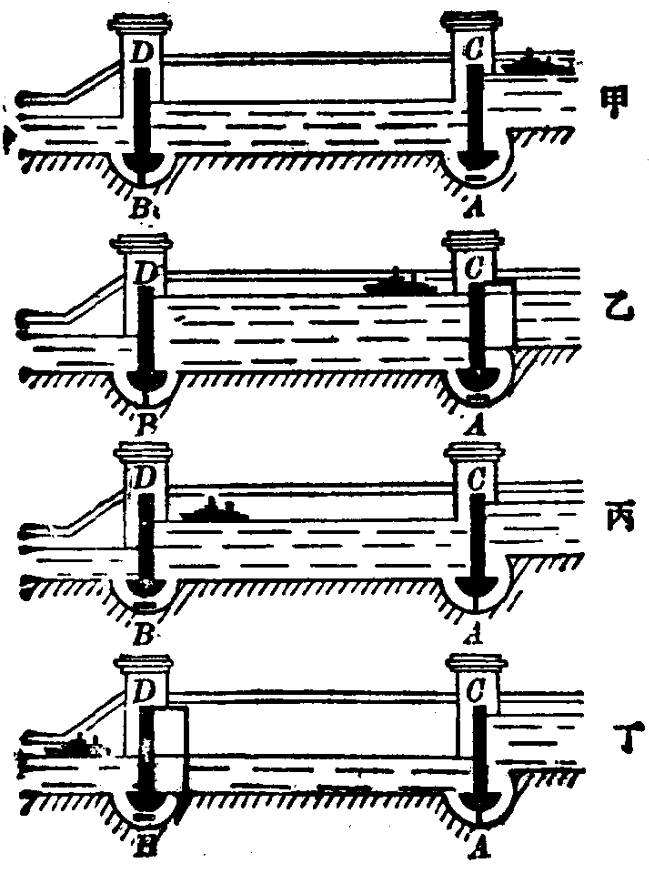
\includegraphics[width=0.6\textwidth]{../pic/czwl1-ch5-34}
    \caption{船通过船闸由上游驶往下游}\label{fig:5-34}
\end{figure}

船只怎样通过船闸呢?比如当船到达上游闸门时,首先关闭下游闸门 $D$ 和阀门 $B$,
打开上游阀门 $A$,让水由上游流进闸室(图 \ref{fig:5-34} 甲)。闸室里的水面就逐渐上升。
等到闸室里的水面跟上游水面相平时,打开上游闸门 $C$,船就可以由上游驶进闸室(图 \ref{fig:5-34} 乙)。
然后关闭上游闸门 $C$ 和阀门 $A$,打开下游阀门 $B$, 让闸室里的水流往下游,闸室里的水面就逐渐下降(图 \ref{fig:5-34} 丙)。
等到闸室里的水面降到跟下游水面相平时,打开下游闸门 $D$,船就可以驶出闸室,开往下游(图 \ref{fig:5-34} 丁)。

船由下游驶往上游的步骤跟上面说的相反。

我国在不少水上运输频繁的江河上修建拦河坝时都同时修建了船闸。
目前最大的是长江葛洲坝船闸,它共有三个船闸,其中的二号、三号船闸已于 1981 年建成通航。
二号船闸的闸室长 280 米, 宽 34 米,能够通过万吨船队。
它的下游闸门高 34 米,每门宽 19.7 米,质量 600 吨,闸门和阀门的开关都由电气设备集中控制,动作灵活。
葛洲坝船闸是世界上少有的巨型船闸之一。



\lianxi

(1) 图 \ref{fig:5-35} 表示啧泉的成因,$AB$ 表示含水层的水面高度,$C$ 和 $D$ 表示不透水的地层,如果在 $C$ 层有空隙,
就会有泉水从这里喷出来,为什么?

\begin{figure}[htbp]
    \centering
    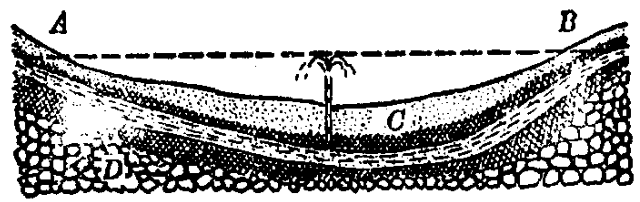
\includegraphics[width=0.6\textwidth]{../pic/czwl1-ch5-35}
    \caption{喷泉的成因示意图}\label{fig:5-35}
\end{figure}

(2) 图 \ref{fig:5-36} 是简易自来水设备的示意图,水塔中的水箱必须比装有水笼头的建筑物高,为什么?

\begin{figure}[htbp]
    \centering
    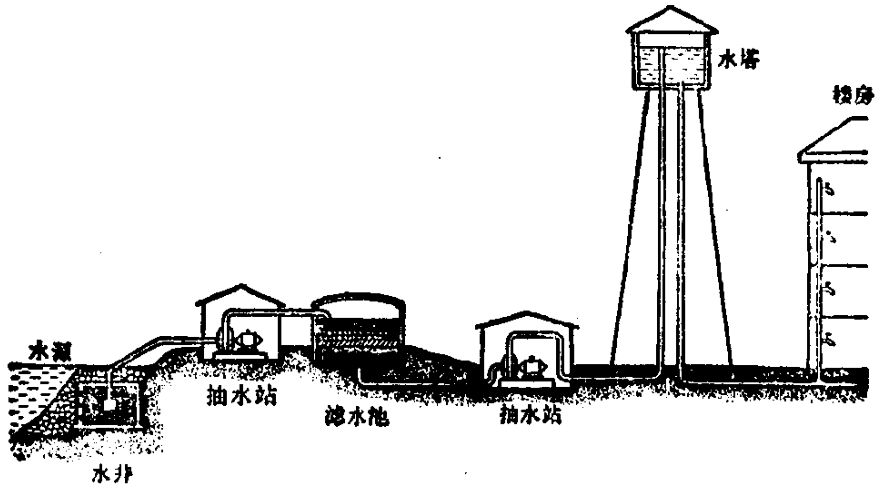
\includegraphics[width=0.6\textwidth]{../pic/czwl1-ch5-36}
    \caption{简易自来水设备示意图}\label{fig:5-36}
\end{figure}

(3) 图 \ref{fig:5-37} 是牲畜自动喂水器的示意图,饮水杯 $A$、$B$、$C$ 里的水可以保持一定的水位,供牲畜饮用,说明它的道理。

\begin{figure}[htbp]
    \centering
    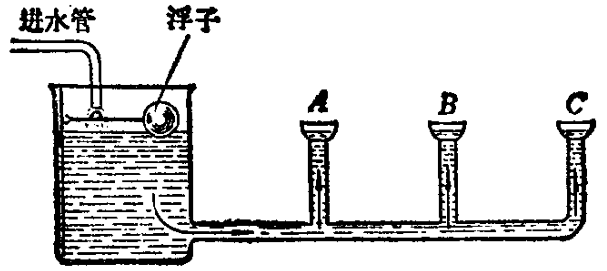
\includegraphics[width=0.6\textwidth]{../pic/czwl1-ch5-37}
    \caption{牲畜自动喂水器示意图}\label{fig:5-37}
\end{figure}

(4) 除了书上讲过的,自己再举出几个利用连通器的例子。

